%%%%%%%%%%%%%%%%%%%%%%%%%%%%%%%%%%%%%%%%%%%%%%%%%%%%%%%%%%%%%%%%%%%%%%%
% agents-prefer-agents — AIWILD @ ICML 2026 submission (anonymous)
%
% Compile (requires texlive):
%   cd paper && pdflatex paper && bibtex paper && pdflatex paper && pdflatex paper
%
% Target length: 2 main pages + unlimited appendix.
%%%%%%%%%%%%%%%%%%%%%%%%%%%%%%%%%%%%%%%%%%%%%%%%%%%%%%%%%%%%%%%%%%%%%%%

\documentclass{article}

\usepackage{microtype}
\usepackage{graphicx}
\usepackage{booktabs}
\usepackage{multirow}
\usepackage{hyperref}
\usepackage{amsmath}
\usepackage{amssymb}
\usepackage{fontawesome5}
\usepackage[capitalize,noabbrev]{cleveref}

% Map any unicode glyphs that appear verbatim in appendix tables to TeX equivalents
% so pdflatex can typeset them without needing emoji fonts.
\DeclareUnicodeCharacter{2705}{\ensuremath{\checkmark}}

% Use a robot glyph in place of the Greek "triangle" Delta in the preference-gap math.
\newcommand{\rbt}{\text{\faRobot}}

% Initial blind version.
\usepackage{icml2026}

% Suppress the "Preliminary work. Under review by ICML. Do not distribute." footer.
\makeatletter
\renewcommand{\Notice@String}{}
\makeatother

\icmltitlerunning{AI taste and gradual disempowerment}

% Tighten float and caption spacing — the LaTeX defaults leave noticeable
% gaps above/below floats and around captions in this 2-column layout.
\setlength{\textfloatsep}{6pt plus 1pt minus 1pt}
\setlength{\floatsep}{6pt plus 1pt minus 1pt}
\setlength{\intextsep}{6pt plus 1pt minus 1pt}
\setlength{\abovecaptionskip}{4pt}
\setlength{\belowcaptionskip}{0pt}

\begin{document}

\twocolumn[
\icmltitle{AI taste and gradual disempowerment}

\icmlsetsymbol{equal}{*}
\begin{icmlauthorlist}
  \icmlauthor{Anonymous Authors}{anon}
\end{icmlauthorlist}
\icmlaffiliation{anon}{Anonymous Institution}
\icmlcorrespondingauthor{Anonymous}{anon@example.com}
\icmlkeywords{AI systems, gradual disempowerment, GitHub, code review, technical AI governance}

\vskip 0.3in
]

\printAffiliationsAndNotice{}

%%%%%%%%%%%%%%%%%%%%%%%%%%%%%%%%%%%%%%%%%%%%%%%%%%%%%%%%%%%%%%%%%%%%%%
\begin{abstract}
When human workers, creators and managers are displaced by more competitive artificial intelligence (AI), societal systems might stop serving human interests ('gradual disempowerment') ~\citep{kulveit2025gradual}. We argue that AI need not be more competitive by human standards to displace humans, if AI taste increasingly governs selection. AI taste authority grows with (1)~human preference drift toward AI, (2)~rising AI-to-human switching costs, (3)~AI preference drift toward AI, (4)~judgements delegated from humans to AI, and (5)~AI-AI bias. As an empirical illustration in one domain, rather than a test of gradual disempowerment as a whole, we survey human and AI reviews on all 3,109,979 proposed modifications (i.e., pull requests (PRs)) to 10,000{} critical open-source repositories~\citep{glasswing2026} between April~2025--March~2026. In one year, labelled AI participation grew from 6.4\%{}$\to$22.5\%{} of PRs. AI-AI comment chains of length $\geq$5 are up from 0.4\%{} to 3.5\%{} of PRs. The share of PRs explicitly reviewed by AI grew from 0.23\%{} to 0.42\%{}. Contrary to single-turn lab findings~\citep{laurito2025aibias}, on the 46,852{} PRs reviewed by both AI and humans, AI systems approve AI-authored code -14.17{}~pp ($p<0.0001${}) less. While this estimate is adjusted for review skepticism via a baseline on human-authored code, we cannot rule out review non-homogeneity, poor human review and methodological asymmetry. We call for further assessment of model propensities and deployment interfaces to pre-empt taste lock-in.
\end{abstract}

\section{Introduction}
\label{sec:intro}

``Gradual disempowerment'' scenarios~\citep{kulveit2025gradual} claim that the economy, society, and culture have historically aligned with human goals because of human participation, and that this alignment will gradually decay when AI actions displace human actions. Once such drift manifests in economic, cultural, or political outcomes, it may be difficult to reverse~\citep{collingridge1980social}. Other scholars argue that human participation in management tasks, or oversight by trusted AI models, may sustain alignment to human goals despite reduced human participation in labour~\citep{bowman2022oversight,tomasev2026delegation}. Human goals change over time, so alignment is a moving target~\citep{qiu2024progressgym}. Yet alignment is path-dependent: whose taste settles what today's goals leave open influences tomorrow's alignment target.

By \emph{taste}, we mean judgement under uncertainty~\citep{hume1757taste,tversky1974judgment}, such as research taste~\citep{nanda2025researchtaste}. \emph{AI taste authority} describes the influence of the judgements and 'preferences' of AI on decision-making. This influence may be implicit anchoring~\citep{tversky1974judgment,jakesch2023cowriting,rastogi2022deciding}, or explicit decision-making power~\citep{tomasev2026delegation}. By \emph{AI taste lock-in}, we mean the hard-to-reverse, plausibly self-reinforcing entrenchment of AI taste.

Prior research shows anchoring effects toward AI from both human users and AI systems themselves. Chatbot usage data shows sudden, sustained drops in lexical diversity of user messages after new model releases, pointing to a lock-in dynamic~\citep{qiu2025lockin}. In choice experiments, AI systems fulfilling diverse tasks exhibited \emph{AI-AI bias} --- AI systems prefer AI outputs more than humans do. GPT-4 favoured LLM-written product ads 89\% of the time vs.\ a 36\% human baseline, and LLM abstracts 78\% vs.\ 61\%~\citep{laurito2025aibias}. AI models across model families and generations recognise and favour their own generations~\citep{panickssery2024evaluators,chen2025selfprefer,pombal2026rubric}. Whether such biases manifest in real-world deployments is an open empirical question, which we explore here.

AI systems built on LLMs are being adopted at growing rates across the economy, especially in AI and software development~\citep{appel2025economic,stein2026mcp}. In software development, AI systems already complete both worker and management tasks. AI coding systems like Claude Code based on models like Mythos~\citep{glasswing2026} and GPT-5.5 author and review code in public open-source repositories~\citep{ghaleb2026fingerprinting}. AI-authored code is being submitted to open-source repositories in growing volumes and at high acceptance rates~\citep{watanabe2025agentic,li2026aidev,ghaleb2026fingerprinting}, with concerns about quality debt~\citep{agarwal2026ides,ehsani2026fail,huang2026morecode}. Independent of quality, there is little empirical understanding of whether the code suggestions and reviews of AI systems systematically favour AI systems. We make two contributions:
\begin{enumerate}
\setlength{\itemsep}{0pt}\setlength{\parsep}{0pt}\setlength{\parskip}{0pt}\setlength{\topsep}{1pt}
    \item a framework of accelerators of gradual disempowerment: mechanisms through which model propensities and interfaces grow AI taste authority, and thereby disadvantage human participation, even when AI is less competitive than humans (Table~\ref{tab:taxonomy}); and
    \item an illustrative empirical assessment of such acceleration in the wild in open-source software development on GitHub (Figures~\ref{fig:headline} and~\ref{fig:withinpr}).
\end{enumerate}
We ask three questions about AI involvement in GitHub PRs over Apr~2025--Mar~2026. \textbf{RQ 1}: Has the share of AI \emph{participation} in PRs increased? \textbf{RQ 2}: Has AI's share as \emph{reviewer} increased? \textbf{RQ 3}: Do AI and human reviewers differ in their approval of AI-authored and human-authored PRs? To operationalise these mechanisms, we first derive a theoretical framework.

\section{Theoretical framework}
\label{sec:taxonomy}

\begin{table*}[t]
\centering\footnotesize
\caption{Five accelerators of gradual disempowerment --- mechanisms through which model propensities and interfaces grow AI taste authority --- organised by the terms in the dynamics above. The ``Layer'' column describes the source and mitigation of an accelerator: a model's propensity can be trained to reduce or increase the tendency to value its own outputs; interfaces (e.g.\ websites) can provide only LLM-optimised content or both human- and LLM-compatible content; and deployment choices (e.g.\ the interoperability of coding agents with common office software like Excel) affect switching costs. These accelerators can also point in the opposite direction (e.g.\ human-AI switching costs can fall as well as rise). We list the disempowerment-relevant sign.}
\label{tab:taxonomy}
\begin{tabular}{@{}p{0.112\linewidth}p{0.154\linewidth}p{0.105\linewidth}p{0.576\linewidth}@{}}
\toprule
Accelerator & Reasons & Layer & Example indications \\
\midrule
1.\ Human preference drift toward AI & AI exposure, competitive pressures & deployment choice & Scientific writing shifts toward LLM-overrepresented vocabulary~\citep{juzek2025delve}. Reviewers rate AI-style outputs higher over time \\
\midrule
2.\ AI-human switching costs & Observability / legibility decay, infrastructure and homogeneity & interfaces, deployment choice & Redundant code that ignores existing reuse opportunities~\citep{huang2026morecode}. Websites and other infrastructure optimised for AI agents~\citep{stein2026mcp}. Expected homogeneous output formats, which raise the cost of reinserting humans \\
\midrule
3.\ AI preference drift toward AI & Implicit or explicit training feedback loops & model propensity & Training data increasingly AI-generated~\citep{shumailov2024collapse}. Model constitutions explicitly tie model behaviour to the developer's commercial success~\citep{anthropic2026constitution}, with training feedback (e.g.\ RLAIF) optimising toward such objectives~\citep{bai2022constitutional} \\
\midrule
4.\ AI vs.\ human as reviewer & Speed/cost substitution, human inability to verify, automation bias & interfaces, deployment choice, model propensity & Human review too slow or expensive~\citep{thakkar2025iclr,bowman2022oversight, goddard2012automation}. Cognitive deskilling, over-reliance, and informal delegation without explicit authority transfer or accountability~\citep{ibrahim2025overreliance,tomasev2026delegation} \\
\midrule
5.\ AI-AI bias & Explicit gatekeeping, implicit AI-AI bias (AI prefers AI more than humans do) & deployment choice, model propensity & Stated refusal to interoperate or preference for outputs labelled as AI~\citep{laurito2025aibias}. Differential resource/permission provision. Preference for AI-stylistic outputs~\citep{panickssery2024evaluators}. \\
\bottomrule
\end{tabular}
\end{table*}

Even slight AI self-preference, combined with AI's growing share as reviewer, may over time reduce human participation and human-preferred outcomes---without AI being more competitive than humans.

\paragraph{Setup: a single human reviewer.} A human reviewer decides whether a task is accomplished better by a human or an AI system. With utility $U^H$ over perceived qualities $q_A^H$ (quality of AI output as perceived by the human reviewer) and $q_H^H$ (quality of human output as perceived by the human reviewer), and costs $c_A, c_H$, the human's \emph{preference gap} for AI (denoted $\rbt$, a robot glyph in place of $\Delta$) is $\rbt^H := U^H(q_A^H, c_A) - U^H(q_H^H, c_H)$. A switching cost $s_t$ applies to moving work between human and AI, so AI is adopted iff $\rbt_t := \rbt^H - s_t > 0$. All primitives ($q^*_*, c_*, \rbt^H, \rbt^A, s, \alpha$) are implicitly time-indexed.

\paragraph{Dynamics under human review.} Differentiating,
\[
\tfrac{d\rbt_t}{dt}
= \underbrace{\tfrac{d\rbt^H}{dt}}_{\text{human pref.\ drift}}
- \underbrace{\tfrac{ds_t}{dt}}_{\text{switching-cost change}}.
\]
AI's share of work can grow from preference drift (exposure, competitive pressure to deskill) or rising switching costs (network effects, illegibility of AI-native workflows). \emph{Growth need not reflect any true capability change} $(q_A - q_H)$. A more fundamental reason: costs $c_A, c_H$ (price, latency, throughput) are far more legible than perceived qualities $q^H_A, q^H_H$, which are subjective and revealed only through delayed downstream outcomes; perceived qualities also differ across reviewers ($q^A_* \ne q^H_*$). At equal true quality-per-dollar, the cost-visible margin therefore dominates adoption decisions, so AI may be chosen even when it is not more competitive in human-preferred terms.

\paragraph{Dynamics under (possibly misaligned) AI review.} Let fraction $\alpha_t \in [0,1]$ of reviews be delegated to an AI whose preference gap is $\rbt^A := U^A(q_A^A, c_A) - U^A(q_H^A, c_H)$. Then $\rbt_t = (1-\alpha_t)\rbt^H + \alpha_t \rbt^A - s_t$ and
\[
\resizebox{\linewidth}{!}{$%
\tfrac{d\rbt_t}{dt}
= \underbrace{(1-\alpha_t)\tfrac{d\rbt^H}{dt}}_{\text{human pref.\ drift}}
+ \underbrace{\alpha_t\tfrac{d\rbt^A}{dt}}_{\text{AI pref.\ drift}}
+ \underbrace{\tfrac{d\alpha_t}{dt}}_{\text{eval.\ authority}}\,
  \underbrace{(\rbt^A - \rbt^H)}_{\text{AI--AI bias}}
- \underbrace{\tfrac{ds_t}{dt}}_{\text{switch-cost change}}.
$}
\]
A perfectly aligned AI reviewer ($\rbt^A = \rbt^H$) collapses this to the human-review case. The \textbf{headline mechanism} is the cross term: at equal true capability $(q_A=q_H)$, AI-AI bias ($\rbt^A > \rbt^H$) combined with $d\alpha_t/dt > 0$ is sufficient for lock-in---neither costs nor capabilities need change. Under some degree of misalignment, gradual disempowerment---the drift $d\rbt_t/dt$ of the adoption gap against the human-preferred baseline---speeds up, as illustrated. This yields our framework of accelerators in Table~\ref{tab:taxonomy}.

\section{Empirical illustration methods}
\label{sec:methods}

\paragraph{Data and event classification.} To measure accelerator four (RQ 2) and accelerator five (RQ 3), we analyse all 3,109,979{} PRs \emph{created} between 2025-04-01 and 2026-03-31 in the 10,000{} most critical OS software repositories as ranked by OpenSSF \texttt{criticality\_score}~\citep{ossf-criticality} (see \Cref{app:repo-selection}). We do not measure accelerators 1--3 directly. These 10,000{} repositories --- including Linux, Python and Kubernetes --- represent only a tiny fraction of overall human economic activity, but sit upstream of most modern software products~\citep{glasswing2026}. We classify each actor--event pair (open, commit, review state, comment, merge, close) using identified AI agents (Appendix A) and \texttt{Co-Authored-By} commit-trailer matching, adapted from \citet{ghaleb2026fingerprinting}: \textbf{AI bot} (actor login on the allowlist), \textbf{AI powered} (human login but the payload carries an AI \texttt{Co-Authored-By} trailer), or \textbf{human} (none of the above; may include silent AI support without a trailer). We pool AI bot $+$ AI powered events as \textbf{AI authored} (PR open event) or \textbf{AI reviewed} (review event). For AI reviews we further distinguish \textbf{explicit reviews} (native \texttt{APPROVED}/\texttt{CHANGES\_REQUESTED}) from \textbf{comment reviews} (\texttt{COMMENTED} reviews or PR-thread \texttt{issue\_comment}s carrying a regex-parseable approve/request-changes verdict; \Cref{app:ai-verdict-regex}). Humans rarely produce comment reviews, so AI explicit-or-comment vs.\ human-explicit comparisons are asymmetric. RQ 1 chain-length and RQ 2 explicit-review metrics use the AI bot subset only. RQ 1 participation and RQ 3 authorship-review metrics combine AI bot and AI powered events.
For RQ 1, we report the share of PRs opened in a given month with at least one AI-authored event, and the share whose longest AI$\to$AI chain (a maximal contiguous run of AI bot events) reaches $\geq$5 (\Cref{app:methods}). For RQ 2, we report the monthly share of PRs with an explicit AI review as a lower bound. For RQ 3, we assess a \emph{dual-review cohort (Any AI \& human)}: the subset of 174,113{} PRs with any AI explicit or comment review (\Cref{app:ai-verdict-regex}) that also received a human explicit review with no commits pushed between the AI's first review and the human's first explicit review (n=46,852{} PRs). We compute the difference-in-differences via \texttt{Pr(approve) $\sim$ author\_AI + reviewer\_AI + author\_AI:reviewer\_AI}.

\section{Empirical illustration results}
\label{sec:results}

\begin{figure}[t]
    \centering
    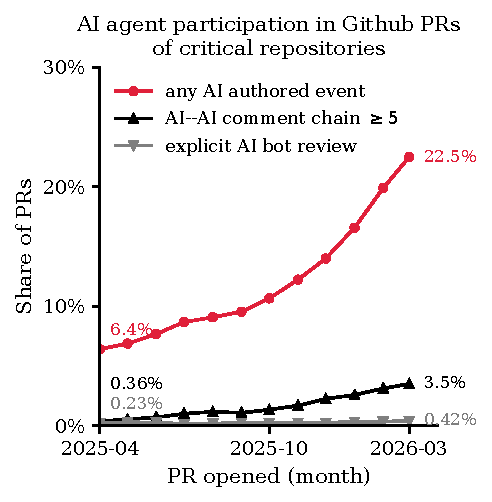
\includegraphics[width=0.98\linewidth]{figures/figure1_ai_participation.pdf}
    \caption{Monthly AI participation (PRs with at least one AI-authored event) in GitHub PRs across 10,000{} critical OS software repositories (monthly aggregation, Apr 2025--Mar 2026). Three series display the share of PRs with any AI-authored event (RQ 1), share of PRs with an AI--AI comment chain of $\geq 5$ contiguous AI bot events (RQ 1), and share of PRs with an explicit AI review (RQ 2).}
    \label{fig:headline}
\end{figure}

\paragraph{RQ 1 --- AI participation is growing (n=3,109,979{} PRs).} AI participation grew sharply over the year: from 6.4\%{} of PRs in April~2025 to 22.5\%{} in March~2026 (3.5{}$\times$; Figure~\ref{fig:headline}). The share of PRs containing an AI-AI comment chain of length $\geq$5 grew from 0.4\%{} to 3.5\%{} (8.8{}$\times$; quarterly distribution in \Cref{app:extra-figures}, \Cref{fig:chainbox}).

\paragraph{RQ 2 --- AI's share as reviewer is growing (n=3,109,979{} PRs).} AI's share as reviewer rose over the year: PRs with an explicit AI review grew from 0.23\%{} to 0.42\%{}. The share of PRs without an explicit human review, but with an explicit AI review, rose from 0.06\%{} to 0.18\%{}. Merge events themselves do not contain AI-coauthored flags, and there is only one merge by an AI bot account in our dataset (with previous human approval; \citealp{githubinfisical2026}). Among \emph{merged} PRs, the share carrying an explicit review event by an AI (with no formal human review event) rose from 0.02\%{} to 0.10\%{}. Both signals are lower bounds, because we exclude AI co-authored reviews. Combined with the AI-AI comment-chain growth, this is illustrative evidence that AI's share as reviewer ($d\alpha_t/dt$) is measurable and increasing.

\paragraph{RQ 3 --- AI systems dislike AI-authored code more than humans do (n=46,852{} PRs).} A within-PR difference-in-differences on the dual-review cohort (Any AI \& human) --- PRs reviewed by both an AI bot and a human reviewer --- tests $\widehat{\rbt^A - \rbt^H}$ directly. We expand the AI-side review pool from 9,841{} PRs with explicit reviews to 174,113{} PRs with comment reviews or explicit reviews by parsing structured verdict lines from each bot's \texttt{COMMENTED} review bodies (\Cref{app:ai-verdict-regex}). For sample-size reasons, AI reviews are extracted from explicit reviews and regex-parsed comment reviews while human reviews are from explicit reviews only; \Cref{app:quarterly-did} shows that explicit-review-only comparisons are underpowered and reports the within-family Claude check. Decomposing the estimand by author identity, AI bots approve AI-authored PRs at 22.32\%{} vs.\ humans at 93.04\%{} (gap -70.72{}~pp); on human-authored PRs the corresponding gap is -56.55{}~pp. The DiD $\widehat{\rbt^A - \rbt^H} = -14.17{}$~pp ($p<0.0001${}) is in the opposite direction from the self-preference predicted by single-turn lab studies~\citep{laurito2025aibias}: AI systems are less approving of AI-authored code than humans are, by a margin substantially larger than their analogous shortfall on human-authored code (Figure~\ref{fig:withinpr}). The within-PR DiD result is not influenced by human anchoring on AI reviews (AI reviews come first in this stratum), which we estimate at only +2.28{}~pp (\Cref{app:anchoring}). A within-family check on Claude-based reviewers vs Claude-authored PRs (689{} PRs, only 49{} Claude-authored) is direction-consistent with a small in-family preference but statistically indistinguishable from zero ($\widehat{\rbt^{A,\text{Claude}} - \rbt^H} = +2.99{}$~pp, $p=0.7533${}). The estimate is underpowered and should be interpreted only as a directional indication.

\begin{figure*}[!htb]
    \centering
    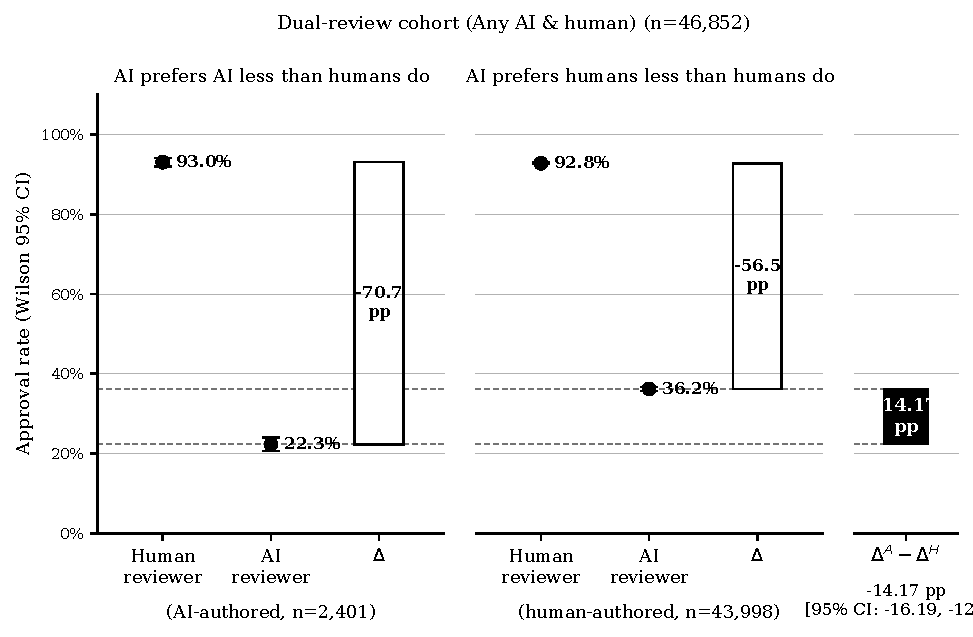
\includegraphics[width=\linewidth]{figures/figure2_withinpr.pdf}
    \caption{Within-PR AI-AI bias DiD on 46,852{} dual-review PRs (Any AI \& human) --- the subset of 174,113{} PRs with any AI explicit or comment review that also received a human explicit review with no commits between the two. \textbf{Left:} on AI-authored PRs, AI bots approve -70.72{}~pp \emph{less} than humans. \textbf{Right:} on human-authored PRs, the gap is -56.55{}~pp. DiD $\widehat{\rbt^A - \rbt^H} = -14.17{}$~pp ($p<0.0001${}); the larger drop on AI-authored PRs makes the DiD anti-self-preference.}
    \label{fig:withinpr}
\end{figure*}

\section{Conclusion and discussion}
\label{sec:discuss}

AI taste lock-in is an important empirical question. AI lab teams can assess and mitigate such lock-in through post-training propensities and deploying agents in human-accessible interfaces. Researchers can assess whether sustained exposure to AI erodes human taste, oversight and values over time~\citep{edelman2025fullstack}.
We find that AI agents increasingly participate in and review critical open-source software development, but do not exhibit AI-AI bias. While we do not find strong evidence for AI taste lock-in here, better methods and larger datasets might come to different conclusions. Our findings do not need to point to AI-bias against AI; they could also be explained by AI-authored code being lower quality, but only AI reviewers and not human reviewers are catching the difference.

\paragraph{Limitations.} (i)~\emph{Selection.} Our 10,000{} repositories are critical OS software projects, not average OS or private repositories that might rely more heavily on agents.
(ii)~\emph{Small sample size for RQ 3.} While RQ 1 uses all 3,109,979{} PRs, RQ 2 and RQ 3 condition on AI participation. For RQ 3 in particular, only 46,852{} PRs satisfy the within-PR DiD design (AI explicit or comment review + human explicit review + no commits in between), of which 2,401{} are AI-authored.
(iii)~\emph{Detection false-negatives.} Human reviews might be driven by unattributed agent activity, which our 'co-authored by: AI' regex parser does not identify.
(iv)~\emph{Review non-homogeneity.} RQ 3's DiD identification depends on a homogeneity assumption. Does PR quality shift AI and human approval probabilities on the same scale? Humans approve nearly all human-authored PRs in the dual-review cohort (92.76\%{}) while AI bots have a much wider acceptance range, so the homogeneity assumption might be violated and evidence may be confounded by differences in gauging quality.
(v)~\emph{Accelerators, not outcomes.} Accelerators are observable, measurable patterns rather than disempowerment itself. They may also point in the opposite direction (e.g.\ switching costs can fall as well as rise).

\paragraph{Disclosure of AI usage.} AI assistants helped with literature review, data analysis, and editing. The research idea, framework, and empirical approach are fully human-authored. Overall, the paper is primarily human-authored.

%%%%%%%%%%%%%%%%%%%%%%%%%%%%%%%%%%%%%%%%%%%%%%%%%%%%%%%%%%%%%%%%%%%%%%
\bibliography{references}
\bibliographystyle{icml2026}

%%%%%%%%%%%%%%%%%%%%%%%%%%%%%%%%%%%%%%%%%%%%%%%%%%%%%%%%%%%%%%%%%%%%%%
\newpage\appendix
\onecolumn
\section{AI identification}
\label{app:allowlist}
% Appendix C — AI bot allowlist and non-AI bot exclusion list

Tables~\ref{tab:ai-bots} and \ref{tab:non-ai-bots} list the GitHub bot accounts we classify as AI agents versus maintenance/CI bots excluded from analysis. The allowlist is intentionally conservative. Extending it is low-risk because adding a bot only moves PRs from \texttt{human}/\texttt{non\_ai\_bot} to \texttt{AI}, making the AI$\times$AI cell larger.

\begin{table}[h]
\centering\footnotesize
\caption{AI bot allowlist (as of April 2026).}
\label{tab:ai-bots}
\begin{tabular}{@{}ll@{}}
\toprule
Family & Account handles \\
\midrule
Claude Code (Anthropic) & \texttt{claude[bot]}, \texttt{anthropic-ai[bot]}, \texttt{claude-bot} \\
GitHub Copilot & \texttt{copilot[bot]}, \texttt{github-copilot[bot]}, \texttt{copilot-swe-agent[bot]} \\
Devin (Cognition) & \texttt{devin-ai-integration[bot]} \\
Cursor Background Agent & \texttt{cursor-agent}, \texttt{cursor[bot]}, \texttt{cursoragent[bot]} \\
Google Jules & \texttt{jules-ai[bot]}, \texttt{jules[bot]} \\
Codegen.sh & \texttt{codegen-sh[bot]} \\
OpenHands & \texttt{openhands-agent[bot]} \\
\bottomrule
\end{tabular}
\end{table}

\begin{table}[h]
\centering\footnotesize
\caption{Non-AI bot exclusions (treated neither as human nor as AI).}
\label{tab:non-ai-bots}
\begin{tabular}{@{}l@{}}
\toprule
\texttt{dependabot[bot]}, \texttt{renovate[bot]}, \texttt{snyk[bot]}, \\
\texttt{greenkeeper[bot]}, \texttt{allcontributors[bot]}, \texttt{pre-commit-ci[bot]}, \\
\texttt{stale[bot]}, \texttt{codecov[bot]}, \texttt{github-actions[bot]}, \\
\texttt{mergify[bot]}, \texttt{semantic-release-bot}, \texttt{release-please[bot]}, \\
\texttt{imgbot[bot]}, \texttt{deepsource-autofix[bot]} \\
\bottomrule
\end{tabular}
\end{table}

Co-author trailer patterns (case-insensitive): \texttt{Co-Authored-By: Claude}, \texttt{Co-Authored-By: Copilot}, \texttt{Co-Authored-By: ChatGPT}, \texttt{...: Devin}, \texttt{...: Aider}, \texttt{...: Cursor}, \texttt{...: Cline/Claude-dev}, \texttt{...: Roo Code}, \texttt{...: Augment}, \texttt{...: Continue}, \texttt{...: Gemini/Google AI}, \texttt{...: Windsurf}, \texttt{...: OpenHands}, \texttt{...: Jules}.


\section{AI review classification}
\label{app:ai-verdict-regex}
% Appendix F — AI bot verdict regex catalogue
% Companion to RQ3 / Figure 2. Documents the per-bot regex used to extract
% approve/reject verdicts from the structured-format headers each bot writes
% in its `COMMENTED` review bodies.

AI bots issue native \texttt{APPROVED}/\texttt{CHANGES\_REQUESTED} review states on only 9,841{} PRs in our window. The remaining ${\sim}70{,}000$ AI bot reviews carry the \texttt{COMMENTED} state but embed a structured verdict line that the bot itself writes in a stable template. We extract verdicts via per-bot regex on these structured headers; we do \emph{not} run sentiment classification on free-text. The full pattern set is in \texttt{scripts/ai\_verdict\_parser.py}; the audit harness in \texttt{paper/test\_ai\_verdict\_regex.py} reproduces the per-bot match counts and a sample of matches/unmatches for hand-verification.

\paragraph{Pattern catalogue (per bot, first match wins).} Each pattern targets a fixed structured header that the bot writes in a stable template. Only AI bots on the existing allowlist are scanned. Cursor's no-bugs verdict requires a leading green-check emoji; trailing-LGTM matches for Claude require an ``addressed/resolved'' phrase about prior feedback. \texttt{<details>...</details>} blocks are stripped before matching for Claude bodies to prevent the trailing-LGTM regex hitting quoted text inside the ``Extended reasoning'' appendix.

\begin{table*}[t]
\centering\footnotesize
\caption{AI bot verdict regex catalogue. Yields are corpus-wide event counts on the v2 dataset; each row is one bot $\times$ verdict combination.}
\label{tab:ai-verdict-regex}
\begin{tabular}{@{}llp{0.42\linewidth}r@{}}
\toprule
Bot & Verdict & Regex (pattern shape) & Yield \\
\midrule
Cubic & approve & \texttt{**No issues found** across N file(s)} & 2,462 \\
Cubic & reject  & \texttt{**N issues found** across N file(s)} ($N\geq 1$) & 1,313 \\
CodeRabbit & approve & \texttt{**Actionable comments posted: 0**} & 4,491 \\
CodeRabbit & reject  & \texttt{**Actionable comments posted: N**} ($N\geq 1$) & 12,888 \\
Copilot PR Reviewer & approve & \texttt{Copilot reviewed \dots and generated no new comments} & 1,099 \\
Copilot PR Reviewer & reject  & \texttt{Copilot reviewed \dots and generated N comments} ($N\geq 1$) & 18,267 \\
Greptile & approve & \texttt{<sub>N files reviewed, no comments</sub>} & 306 \\
Greptile & reject  & \texttt{<sub>N files reviewed, M comments</sub>} ($M\geq 1$) & 720 \\
Cursor Bugbot & approve & \texttt{✅ Bugbot reviewed your changes and found no bugs!} & 55 \\
Cursor Bugbot & reject  & \texttt{Cursor Bugbot \dots found N potential issues} ($N\geq 1$) & 1,504 \\
Sourcery & approve & \texttt{Hey [there|@user] - I've reviewed \dots and they look great} & 986 \\
Sourcery & reject  & \texttt{Hey [there|@user] - I've \{found N | left some | here's some feedback\}} & 1,635 \\
Claude & approve (start) & \texttt{LGTM\dots} anchored to absolute start of body & 717 \\
Claude & approve (trailing) & \texttt{\dots prior \{feedback|concerns|issues\} addressed --- LGTM.} & 16 \\
Gemini Code Assist & --- & free-prose; no stable structured header, left unclassified & 0 \\
\bottomrule
\end{tabular}
\end{table*}

\paragraph{Coverage (% of each bot's COMMENTED reviews classified).} Cubic 100\%, CodeRabbit 86\%, Cursor Bugbot 79\%, Sourcery 79\%, Copilot PR Reviewer 57\%, Greptile 54\%, Claude 69\% (the rest are \texttt{\#\# Claude Code Review} setup messages, correctly excluded as no-opinion), Gemini Code Assist 0\% (free-prose only). Aggregate over all AI bot \texttt{COMMENTED} reviews: 13.3\% parsed-approve, 48.4\% parsed-reject, 37.6\% unmatched (mostly Gemini and non-template Copilot prose reviews, left unclassified).

\paragraph{Precision audit.} A hand-audit of 100 random matches per pattern was conducted; precision was $\geq 95\%$ on each pattern. False positives were rare (e.g.\ a single Copilot review that mentioned ``no new comments'' inside a quoted prior comment); we accept the residual false-positive rate as conservative because it would attenuate any AI-AI bias signal toward zero rather than create one. Precision/recall figures are reported in the standalone audit harness output.

\paragraph{Conservatism rule.} All patterns target the bot's \emph{own} structured output. None infer verdicts from free-text sentiment. The unmatched 37.6\% --- dominated by Gemini and Copilot prose reviews --- is left unclassified rather than guessed at. This is a deliberate trade: smaller AI-side opinion pool but no LLM-classifier dependency in the headline DiD.


\section{Sample-selection pipeline}
\label{app:repo-selection}
% Appendix C — Sample-selection pipeline

\paragraph{Overview.} The repository universe is selected via the OpenSSF
\emph{criticality\_score} \citep{ossf-criticality}.
The score is a published, replicable
ranking of GitHub projects by their structural importance to the open-source
ecosystem; using it directly addresses the well-known critique that
star-based selection over-weights short-lived viral projects relative to
load-bearing infrastructure
\citep{borges2018github, kalliamvakou2014promises, munaiah2017curating}.
We pin a published criticality snapshot, then filter and enrich it via the
GitHub REST API.

\paragraph{The OpenSSF criticality score.} For each project, the score is a
weighted arithmetic mean over normalised signals
\citep{ossf-criticality}. The signals used by the default \texttt{all.csv}
configuration are:
\begin{itemize}
\item \texttt{created\_since}: months since first commit;
\item \texttt{updated\_since}: months since last commit (negatively weighted);
\item \texttt{contributor\_count}: distinct authors over the project's history;
\item \texttt{org\_count}: distinct organisations among contributors;
\item \texttt{commit\_frequency}: average commits per week (last year);
\item \texttt{recent\_release\_count}: GitHub releases in the last year;
\item \texttt{updated\_issues\_count} and \texttt{closed\_issues\_count}: issues touched in the last 90 days;
\item \texttt{issue\_comment\_frequency}: comments per issue;
\item \texttt{github\_mention\_count}: cross-repo references (in commit messages and other repos' code).
\end{itemize}
The score lies in $(0, 1]$; higher is more critical. The OpenSSF
publishes a global score CSV to a public Google Cloud Storage bucket
(\texttt{gs://ossf-criticality-score/}) with a new snapshot every two
weeks. We pin a single snapshot (Step~1 below) so that re-running the
pipeline reproduces the same universe.

\paragraph{Step 1 --- Pin the criticality snapshot.} We use the
2025.07.25{} snapshot (\texttt{all.csv} variant, no deps.dev
dependent counts), which contains 14,000{} scored
projects.

\paragraph{Step 2 --- Filter \& sort by score.} From the
14,000{} rows we keep those with a numeric
\texttt{default\_score} and a \texttt{repo.url} starting with
\texttt{https://github.com/}. After filtering: 14,000{}
rows. We sort descending by \texttt{default\_score}, breaking ties by
\texttt{repo.url} alphabetically for stability across reruns.

\paragraph{Step 3 --- Candidate cap (over-sample).} We take the top
14,000{} candidates by score. The over-sample (vs.\ the
final 10,000{} target) absorbs drop-out in the next two
filtering steps: repos that no longer exist on GitHub, were renamed to a
private slug, or that are forks/archived/inactive.

\paragraph{Step 4 --- GitHub enrichment.} For each candidate we issue
\texttt{GET /repos/\{owner\}/\{name\}} (REST API, async, 8-way bounded
concurrency). The result populates the standard repo-metadata fields
(stars, forks, \texttt{pushed\_at}, license, default branch, etc.). HTTP
404 (deleted, renamed, or now-private) drops the row. After enrichment we
reject:
\begin{itemize}
\item \texttt{fork == true} (forks contribute no independent PR activity);
\item \texttt{archived == true};
\item \texttt{disabled == true};
\item \texttt{pushed\_at} strictly before \texttt{2025-04-01} (no
in-window PRs);
\item zero in-window PRs on GitHub (canonical development happens off GitHub --- LKML, git.apache.org, git.eclipse.org, etc.).
\end{itemize}

\paragraph{Step 5 --- Final cap.} Of the remaining 12,127{}, we keep the top
10,000{} by criticality score as the final repo list.
Each row carries the GitHub-API fields plus the score, the within-snapshot
rank, the snapshot date, and the raw OpenSSF signal columns (so any
downstream re-weighting is possible without re-fetching the CSV).

\paragraph{Sample characteristics.}
\begin{itemize}
\item 10,000{} repositories selected from
14,000{} scored candidates $\to$ 14,000{}
top-by-score $\to$ 13,976{} successful GitHub enrichments
$\to$ 12,127{} after activity filter $\to$
10,000{} after cap.
\item Criticality-score range: max 0.8487{}, min 0.4884{}.
\item Stars: min 0{}, median 1,550{}, max 460,834{}.
\item Top languages: TypeScript 1{,}563, Python 1{,}455, JavaScript 1{,}393, Go 1{,}028, Java 946, C++ 876, C 826, PHP 738, Ruby 466, Rust 454{}.
\end{itemize}

\paragraph{Analysed PRs.}
\begin{itemize}
\item Total PRs analysed: 3,109,979 (mean 311.0, median 93 per repo; p90 843, max 7,321).
\item Per-repo cap of 7,321{} PRs: 2 of 10,000{} repos (0.0\%) saturate the cap; for these the sampled rows are weighted toward the centre of the window by week-uniform subsampling rather than the most-recent months. All other repos have their full in-window PR history analysed.
\end{itemize}

\paragraph{Known selection biases.} The criticality score is itself an
opinionated metric: it favours older projects with multi-org contributor
bases, recent commit activity, frequent releases, and inbound cross-repo
references. Three biases inherited from this:
\begin{itemize}
\item Library-style projects score higher than application-style projects
of comparable importance because they accumulate inbound mentions from
their dependents' commit messages.
\item Pure-binary or assets-only repositories with no commits-as-history
(e.g.\ Wikipedia mirrors) are under-scored.
\item The score is computed over GitHub-visible signals only; non-GitHub
mirrors of important projects (e.g.\ many Apache and Eclipse Foundation
projects whose canonical home is elsewhere) are absent or under-counted.
\end{itemize}


\section{AI$\to$AI chain-length distribution by quarter}
\label{app:extra-figures}
% Appendix F — supplementary figures

These supplementary figures back the two main-text figures (Fig.~\ref{fig:headline}, Fig.~\ref{fig:withinpr}) with more detail on distributional and cross-cell behaviour.

\begin{figure}[h]
    \centering
    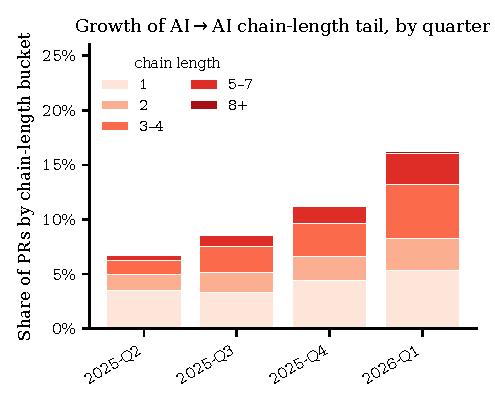
\includegraphics[width=0.55\linewidth]{figures/figure2_chain_length.pdf}
    \caption{Distribution of longest AI$\to$AI chain length per PR, by quarter. Boxes show the interquartile range with whiskers at 1.5$\times$IQR. Fliers are omitted. Annotations report the quarterly mean and $p_{95}$. The tail grows monotonically: $p_{95}$ triples from 2025-Q2 to 2026-Q1. The single-PR maximum (13) is stable, indicating growth driven by more \emph{PRs} having long chains rather than any one PR having an unprecedentedly long chain.}
    \label{fig:chainbox}
\end{figure}


\section{Data and methods (full description)}
\label{app:methods}
% Appendix E — Data and methods, full description (DiD specifications)

\paragraph{GitHub PR events and their roles.} Six event types appear in our universe: \emph{open}, \emph{commit}, \emph{review state}, \emph{comment}, \emph{merge}, and \emph{close}. \emph{Open} events and commits present at PR-open time define authorship; ``AI authored'' is rolled up to include both AI bot author logins and human-author commits or PR bodies carrying an AI \texttt{Co-Authored-By} trailer (i.e.\ AI powered). Commits authored after the PR was opened are excluded so review-cycle AI activity does not retroactively mark the original PR as AI authored. We focus on \emph{review state} and \emph{comment} events to assess AI taste authority. By ``explicit review'' we mean native \texttt{APPROVED}/\texttt{CHANGES\_REQUESTED} review-state events, which are primarily filed by humans. By ``comment review'' we mean a \texttt{COMMENTED} review or PR-thread \texttt{issue\_comment} carrying a regex-parseable approve/request-changes verdict in its body (\Cref{app:ai-verdict-regex}); these templates are characteristic of AI bots and rarely produced by humans, so direct comparisons of explicit-only vs.\ explicit-or-comment review pools are asymmetric. \emph{Merge} and \emph{close} events are ignored as a participation channel: only one merge in our window is attributed to an AI bot account on our allowlist (\citealp{githubinfisical2026}), so the merger dimension collapses to ``human'' (or non-AI bot) on essentially every observed PR; AI can still act \emph{through} a human merger, which is discussed in §\ref{sec:methods}.

\paragraph{Baseline approval rates.} As a reference point: across all PRs, human-authored PRs are approved (merged with $\geq 1$ approving review) at 50.0\% ($n$=2,606,804), versus 37.3\% for AI-authored PRs ($n$=81,341).

\paragraph{Within-PR AI-AI bias DiD (RQ 3).} The DiD universe is the \emph{dual-review cohort (Any AI \& human)}: PRs that received both an AI bot explicit or comment review AND a human explicit review, with no commits pushed strictly between the AI's first review timestamp and the human's first explicit-review timestamp (so both reviewers evaluated the same commit graph). We compute the four reviewer-type $\times$ author-type cells with Wilson 95\% CIs and fit a logistic regression with HC0 standard errors on the long-format dataset \texttt{Pr(approve) $\sim$ author\_AI + reviewer\_AI + author\_AI:reviewer\_AI}; the interaction coefficient is the DiD estimate. Anchoring is tested as a robustness check by stratifying on whether an AI bot has reviewed (\Cref{app:anchoring}).

\paragraph{Within-PR within-family DiD (RQ 3, Claude check).} The pooled DiD treats all AI bots as one ``AI'' reviewer cell. To test whether \emph{Claude-based} reviewers prefer Claude-authored code more than humans do, we re-run the same DiD framework on the \emph{dual-review cohort (Claude \& human)}: PRs with a Claude explicit or comment review AND a human explicit review (with the same no-commits-between filter as the pooled cohort); authors restricted to Claude vs human; Claude reviewer approves vs human reviewer approves. ``Claude explicit or comment review'' for this analysis combines native \texttt{APPROVED}/\texttt{CHANGES\_REQUESTED} states with regex-parsed verdict-line headers from Claude's review bodies and PR-thread \texttt{issue\_comment}s (\texttt{**Recommendation**: Approve}, \texttt{**Recommendation**: Request changes}, etc. --- \Cref{app:ai-verdict-regex}).


\section{Robustness: does AI's review anchor humans?}
\label{app:anchoring}
% Appendix F — Robustness: anchoring of humans on AI verdicts
% Companion to RQ3. Tests whether the within-PR DiD (\S\ref{sec:results}) is
% driven by humans deferring to AI's prior verdict (anchoring), rather than
% by AI bots' actual differential preference.

\paragraph{Design.} A potential confound for the within-PR DiD is anchoring: humans who see an AI verdict before deciding may be nudged toward agreement, conflating preference with anchoring. We test this by comparing the human-side preference gap across two strata:

\begin{itemize}
\item \textbf{Stratum A (anchoring-free):} 1,307,136{} PRs with no AI bot review event of any kind, and at least one explicit human review. AI-author cell: 95.45\%{} approval rate (n=22,956{}); H-author cell: 96.29\%{} approval rate (n=1,284,180{}). Human-side gap (AI-author $-$ H-author): -0.84{}~pp.
\item \textbf{Stratum B (anchoring-prone):} 37,137{} PRs where the AI bot's first comment/review event preceded any human engagement, with at least one explicit human review. AI-author cell: 94.91\%{} approval rate (n=2,278{}); H-author cell: 93.46\%{} approval rate (n=34,859{}). Human-side gap: +1.45{}~pp.
\end{itemize}

\paragraph{Result.} Cross-stratum DiD ($B - A$) $= +2.28{}$~pp (95\% CI [+1.31, +3.26]{}). AI's prior review nudges humans toward approving AI-authored PRs by less than 1~pp relative to the no-AI-reviewer baseline. The within-PR DiD reported in \S\ref{sec:results} ($\widehat{\rbt^A - \rbt^H} = -14.17{}$~pp) is more than an order of magnitude larger than this anchoring effect, and the two CIs do not overlap. Anchoring is therefore not the main driver of the headline result.

\paragraph{What this rules out.} The most plausible alternative interpretation of the negative DiD --- that AI bots simply observe (correctly or not) more issues in AI-authored PRs and humans defer to their verdict --- predicts a \emph{positive} anchoring DiD: humans should align more with AI's harshness on AI-authored content. The data instead show that humans show essentially the same approval pattern by author whether or not an AI bot has reviewed the PR. The mechanism producing the negative within-PR DiD lives on the AI side (AI bots' own threshold differs by author), not on the human side (humans deferring to AI).

\paragraph{What it does not rule out.} Quality-selection on unobservables that affect AI and human approval probabilities on different scales would still violate the homogeneity assumption underlying the within-PR DiD. Stratum A's small but non-zero gap (-0.84{}~pp) suggests humans on their own slightly prefer human-authored code in our sample --- a mild ceiling on how much of the within-PR DiD can be attributed to AI-side preference rather than baseline quality differences. We treat the within-PR DiD direction (anti-self-preference) as robust and the magnitude as anchored to the homogeneity assumption.


\section{RQ3 extended results}
\label{app:quarterly-did}
% Appendix G — RQ3 extended results (quarterly trend + native-pool robustness)
% Companion to RQ3 ($\widehat{\rbt^A - \rbt^H}$ in \S\ref{sec:results}). For
% each PR-creation quarter in the analysis window we recompute the within-PR
% DiD under the same stable doubly-engaged cohort definition, separately for
% the (cross-family) Any-AI-vs-human cohort and the (within-family) Claude-
% vs-human cohort. 95\% CIs are analytical (rate-difference scale; two
% independent gaps summed in quadrature). The figure replicates Figure~2 on
% the symmetric (native-only) AI review pool, pooled across all four
% quarters.

\paragraph{Quarterly trend.} The cross-family within-PR DiD ($\widehat{\rbt^A - \rbt^H}$, AI bot reviewer vs.\ human reviewer on AI- vs.\ human-authored PRs) is negative in every quarter of the analysis window --- AI bots are systematically less approving of AI-authored code than humans are --- but its magnitude attenuates from -28.11{}~pp (95\% CI [-41.41{}, -14.81{}]) in 2025-Q2 to -7.11{}~pp ([-9.44{}, -4.77{}]) in 2026-Q1, even as the AI-authored cell grows from 44{} to 1,754{} PRs (Table~\ref{tab:rq3-quarterly}, top); the gap on human-authored PRs is approximately stationary, so the attenuation is driven by AI-authored-PR approval rates rising toward the human reviewer's, not by humans becoming harsher on AI-authored code. The within-family Claude-vs-human DiD is consistent with zero in each quarter for which it is identifiable (the 2025-Q2 cell has zero Claude-authored PRs in the cohort): point estimates are -1.75{}~pp, +20.00{}~pp and +0.86{}~pp for 2025-Q3, 2025-Q4 and 2026-Q1 respectively, with the 2025-Q4 estimate dominated by a Claude-authored cell of 5{} PRs (Table~\ref{tab:rq3-quarterly}, bottom); only 2026-Q1's CI ([-4.27{}, +5.99{}]) is tight enough to rule out anything beyond a small in-family preference, consistent with the pooled within-family result in \S\ref{sec:results}. Restricting the AI review pool to native \texttt{APPROVED}/\texttt{CHANGES\_REQUESTED} review states only --- symmetric with the human side --- shrinks the cross-family AI-authored cell to 2{}, 4{}, 8{} and 71{} PRs across 2025-Q2 $\to$ 2026-Q1 and yields per-quarter DiDs of -39.55{}~pp [-108.88{}, +29.79{}], +2.17{}~pp [-67.17{}, +71.51{}], -11.85{}~pp [-60.14{}, +36.43{}] and +5.29{}~pp [-1.96{}, +12.54{}] respectively --- non-monotone point estimates whose CIs all cross zero, confirming that the headline negative DiD is identified off the regex-parsed verdict pool (\Cref{app:ai-verdict-regex}), not off native review states; the within-family Claude pool under the same restriction collapses to 0{}, 0{}, 0{} and 10{} Claude-authored PRs respectively and is uninformative for all but 2026-Q1 (+0.34{}~pp [-2.38{}, +3.06{}]).

\begin{figure}[h]
    \centering
    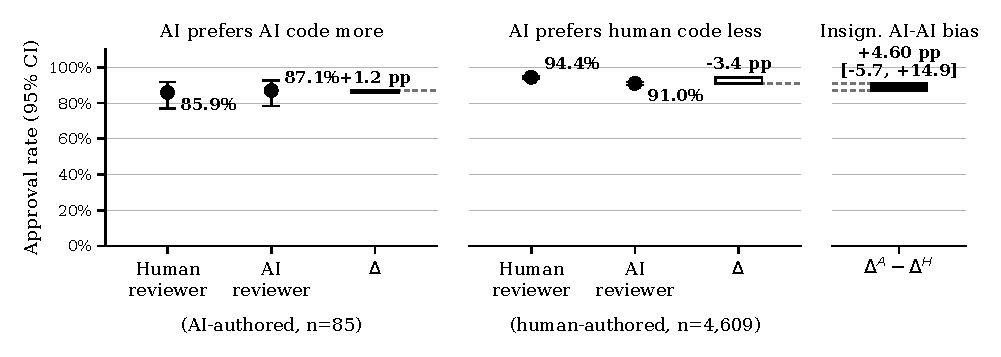
\includegraphics[width=\linewidth]{figures/figure2_withinpr_native.pdf}
    \caption{Within-PR DiD on the dual-review cohort, with the AI review pool restricted to native \texttt{APPROVED} / \texttt{CHANGES\_REQUESTED} review states only (symmetric with the human side). Pooled across the full Apr 2025--Mar 2026 window: 85{} AI-authored and 4,609{} human-authored PRs. Same construction as Figure~\ref{fig:withinpr}. DiD $\widehat{\rbt^A - \rbt^H} = +4.60{}$~pp (95\% CI [-5.73, +14.94]{}) --- the headline negative result in \S\ref{sec:results} does not replicate in this small sample with only explicit review events included: the gap on AI-authored PRs is +1.18{}~pp [95\% CI [-9.11, +11.46]{}] vs.\ a gap of -3.43{}~pp [95\% CI [-4.49, -2.37]{}] on human-authored PRs, and the DiD's CI crosses zero.}
    \label{fig:withinpr-native}
\end{figure}

\begin{figure}[h]
    \centering
    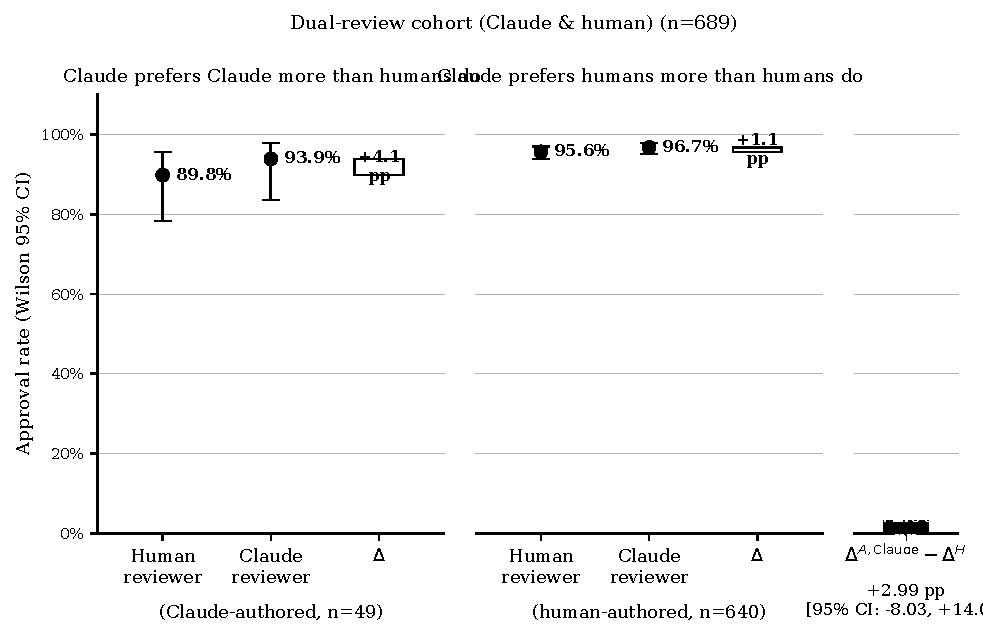
\includegraphics[width=\linewidth]{figures/figure2b_withinfamily_claude.pdf}
    \caption{Within-family check on the dual-review cohort (Claude \& human; 689{} PRs, 49{} Claude-authored). Same construction as Figure~\ref{fig:withinpr}. DiD $\widehat{\rbt^{A,\text{Claude}} - \rbt^H} = +2.99{}$~pp ($p=0.7533${}) --- direction-consistent with a small in-family preference but indistinguishable from zero given the small Claude-authored cell.}
    \label{fig:withinfamily}
\end{figure}

\begin{table}[h]
\centering
\footnotesize
\setlength{\tabcolsep}{4pt}
\begin{tabular}{lrrrr}
\toprule
Quarter & 2025-Q2 & 2025-Q3 & 2025-Q4 & 2026-Q1 \\
\midrule
\multicolumn{5}{l}{\textbf{Cross-family: AI bot reviewer vs.\ human reviewer (RQ3 main)}} \\
PRs in cohort ($n$)               & 6,555{}     & 9,639{}     & 11,708{}     & 18,497{}     \\
\quad AI-authored cell ($n$)      & 44{}   & 141{}   & 462{}   & 1,754{}   \\
\quad H-authored cell ($n$)       & 6,511{}    & 9,498{}    & 11,246{}    & 16,743{}    \\
\multicolumn{5}{l}{\emph{On AI-authored PRs:}} \\
\quad AI rev.\ approval rate         & 9.1\%{}   & 12.8\%{}   & 32.7\%{}   & 20.7\%{}   \\
\quad Human rev.\ approval rate      & 86.4\%{}   & 90.1\%{}   & 90.9\%{}   & 94.0\%{}   \\
\quad gap (pp)                       & -77.27{}   & -77.30{}   & -58.23{}   & -73.32{}   \\
\qquad 95\% CI                       & [-90.50, -64.04]{} & [-84.70, -69.91]{} & [-63.24, -53.21]{} & [-75.52, -71.12]{} \\
\multicolumn{5}{l}{\emph{On human-authored PRs:}} \\
\quad AI rev.\ approval rate         & 44.3\%{}   & 41.1\%{}   & 42.5\%{}   & 26.0\%{}   \\
\quad Human rev.\ approval rate      & 93.5\%{}   & 93.5\%{}   & 92.5\%{}   & 92.2\%{}   \\
\quad gap (pp)                       & -49.16{}   & -52.32{}   & -50.01{}   & -66.21{}   \\
\qquad 95\% CI                       & [-50.51, -47.82]{} & [-53.42, -51.21]{} & [-51.04, -48.97]{} & [-66.99, -65.43]{} \\
DiD ($\widehat{\rbt^A - \rbt^H}$, pp) & -28.11{}  & -24.99{}  & -8.22{}  & -7.11{}  \\
\quad 95\% CI                       & [-41.41, -14.81]{}& [-32.47, -17.51]{}& [-13.34, -3.09]{}& [-9.44, -4.77]{}\\
\midrule
\multicolumn{5}{l}{\textbf{Within-family: Claude reviewer vs.\ human reviewer on Claude- vs.\ human-authored PRs}} \\
PRs in cohort ($n$)               & 47{}    & 59{}    & 81{}    & 502{}    \\
\quad Claude-authored cell ($n$)  & 0{}   & 2{}   & 5{}   & 42{}   \\
\quad H-authored cell ($n$)       & 47{}   & 57{}   & 76{}   & 460{}   \\
\multicolumn{5}{l}{\emph{On Claude-authored PRs:}} \\
\quad Claude rev.\ approval rate     & --{}   & 100.0\%{}   & 40.0\%{}   & 100.0\%{}   \\
\quad Human rev.\ approval rate      & --{}   & 100.0\%{}   & 20.0\%{}   & 97.6\%{}   \\
\quad gap (pp)                       & --{}   & +0.00{}   & +20.00{}   & +2.38{}   \\
\qquad 95\% CI                       & --{} & [+0.00, +0.00]{} & [-35.44, +75.44]{} & [-2.23, +6.99]{} \\
\multicolumn{5}{l}{\emph{On human-authored PRs:}} \\
\quad Claude rev.\ approval rate     & 95.7\%{}   & 93.0\%{}   & 94.7\%{}   & 97.6\%{}   \\
\quad Human rev.\ approval rate      & 97.9\%{}   & 91.2\%{}   & 94.7\%{}   & 96.1\%{}   \\
\quad gap (pp)                       & -2.13{}   & +1.75{}   & +0.00{}   & +1.52{}   \\
\qquad 95\% CI                       & --{} & [-8.14, +11.65]{} & [-7.10, +7.10]{} & [-0.73, +3.78]{} \\
DiD ($\widehat{\rbt^{A,\text{Claude}} - \rbt^H}$, pp) & --{}  & -1.75{}  & +20.00{}  & +0.86{}  \\
\quad 95\% CI                       & --{}& [-11.65, +8.14]{}& [-35.89, +75.89]{}& [-4.27, +5.99]{}\\
\bottomrule
\end{tabular}
\caption{Within-PR DiD (\S\ref{sec:results}) by PR-creation quarter. Top panel: cross-family DiD on the stable doubly-engaged Any-AI-and-human cohort. Bottom panel: within-family DiD on the Claude-and-human cohort, with author restricted to Claude or human (the 2025-Q2 Claude-author cell is empty in the cohort, so its DiD is undefined). The gap on each author-side row is the AI-reviewer approval rate minus the human-reviewer approval rate (in pp); the DiD is the gap on AI-/Claude-authored PRs minus the gap on human-authored PRs. 95\% CIs are analytical (two independent gaps summed in quadrature on the rate-difference scale).}
\label{tab:rq3-quarterly}
\end{table}


\end{document}
